\documentclass{standalone}
\usepackage{textcomp}
\usepackage[dvipsnames]{xcolor}
\usepackage{amsopn, amsmath, amssymb}
\usepackage{booktabs}

\newcommand{\myproc}[1]{\text{\textsc{\text{#1}}}}
\newcommand{\myvar}[1]{\text{\sl #1}}

\usepackage{tikz}
\usepackage{tikz-qtree}
\usepackage{pgfplots}

\usetikzlibrary{
	positioning, 
	matrix, 
	calc,
	arrows,
	shapes,
	fit,
	decorations,
	decorations.pathmorphing
}

\tikzset{
	every picture/.style={
		line width=.4mm,
		text=mc,
		draw=mc,
	},
}

\tikzstyle{arraynodes} = [
	minimum size=5mm, 
	inner sep=0mm,
	anchor=center,
	draw=mc,
	text=mc
]

\tikzstyle{array} = [
	draw=none,
	matrix of nodes,
	nodes={arraynodes},
	ampersand replacement=\&,
	line width=.3mm,
	row sep=-\pgflinewidth,
	column sep=-\pgflinewidth,
]

\tikzstyle{h}=[arraynodes, fill=hcfill]

\newcommand{\logo}{
	\path[use as bounding box] (-2.6, -2.6) rectangle (2.6, 2.6);
	\draw[rounded corners] (-2.5, -2.5) rectangle (2.5, 2.5);
}

\newenvironment{pseudocode}
	{\hrule\medskip}
	{\medskip\hrule}

\colorlet{mc}{white!70!black} % main color
\colorlet{hc}{yellow} % highlight color
%\colorlet{mc}{black} % main color
%\colorlet{hc}{red!90!black} % highlight color

\begin{document}
	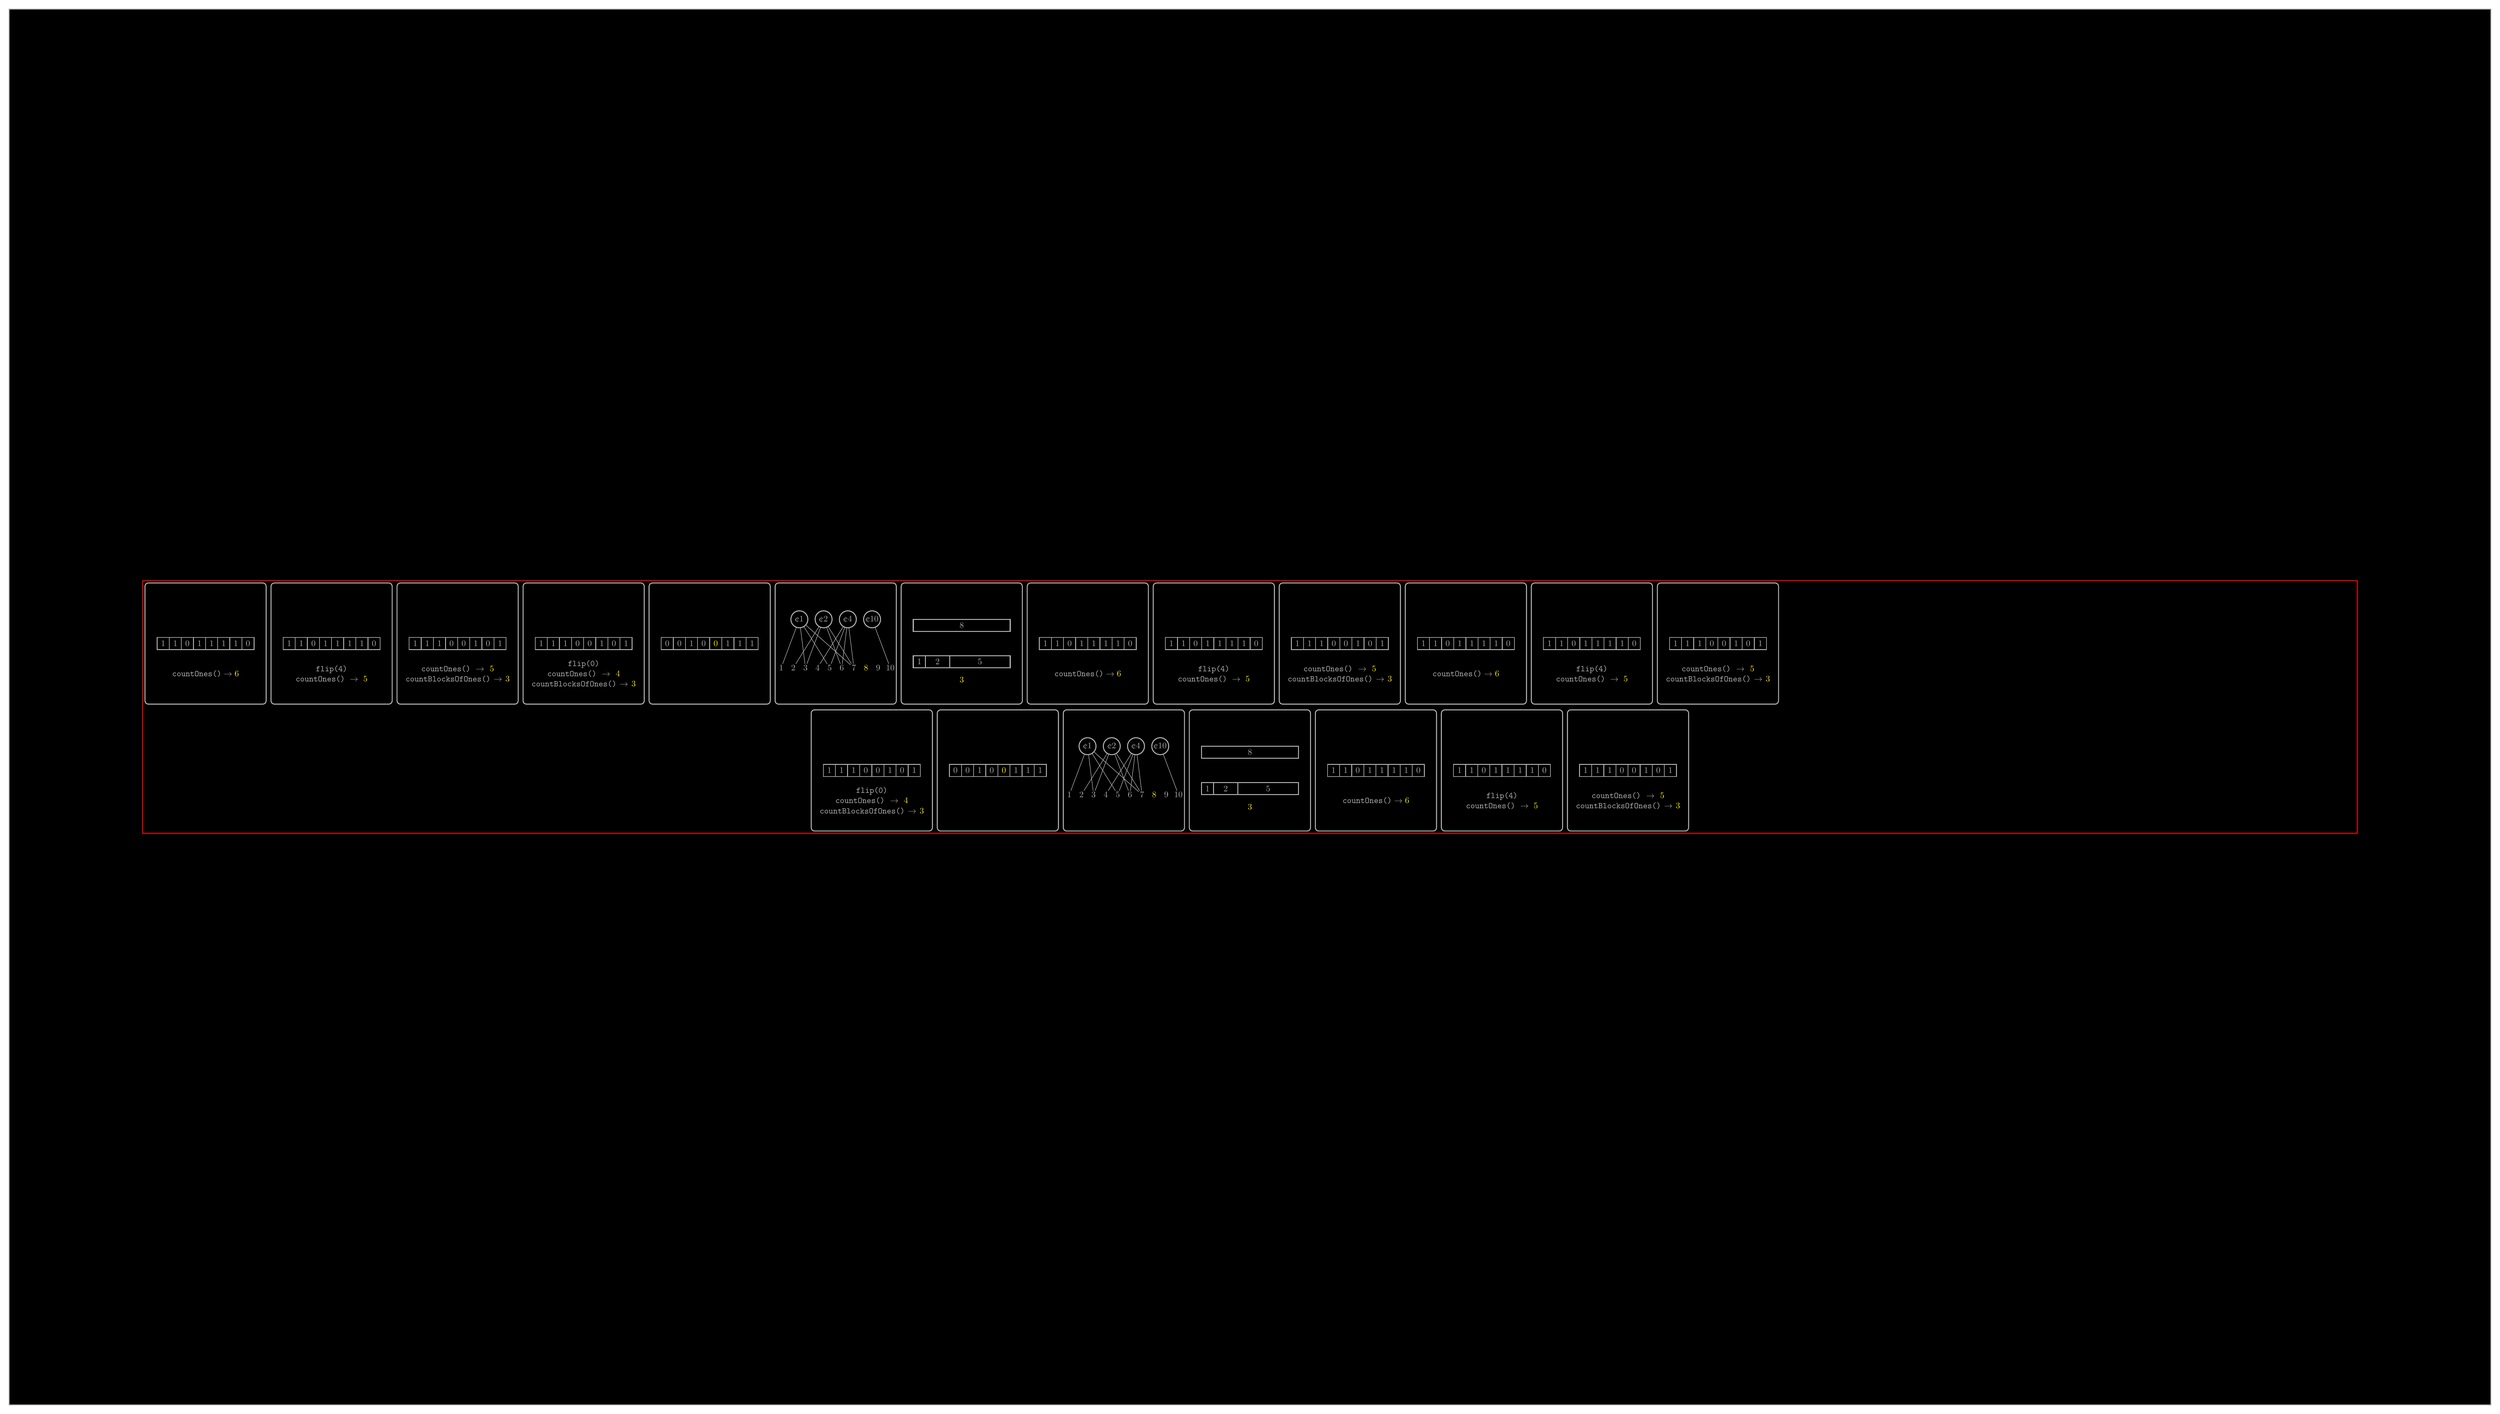
\begin{tikzpicture}
		\filldraw[fill=black] (0, 0) rectangle (2048/20, 1152/20);
		\node[inner sep=0mm, text width=2600, draw=red, align=center] at (2048/40, 1152/40) {
			\tikz{\logo{}
\matrix[array] {1\&1\&0\&1\&1\&1\&1\&0\\};
\node at (0,-1.25) {$\texttt{countOnes()} \to \textcolor{hc}{6}$};}%
			\tikz{\logo{}
\matrix[array] {1\&1\&0\&1\&1\&1\&1\&0\\};
\node[text width=45mm, align=center] at (0,-1.25) {
	$\texttt{flip(4)}$\\
	$\texttt{countOnes()} \to \textcolor{hc}{5}$
};}%
			\tikz{\logo{}
\matrix[array] {1\&1\&1\&0\&0\&1\&0\&1\\};
\node[align=center, text width=48mm] at (0,-1.25) {
	$\texttt{countOnes()} \to \textcolor{hc}{5}$\\
	$\texttt{countBlocksOfOnes()} \to \textcolor{hc}{3}$\\
};}%
			\tikz{\logo{}
\matrix[array] {1\&1\&1\&0\&0\&1\&0\&1\\};
\node[align=center, text width=48mm] at (0,-1.25) {
	$\texttt{flip(0)}$\\
	$\texttt{countOnes()} \to \textcolor{hc}{4}$\\
	$\texttt{countBlocksOfOnes()} \to \textcolor{hc}{3}$\\
};}%
			\tikz{\logo{}
\matrix[array] (a) {0\&0\&1\&0\&|[text=hc]|0\&1\&1\&1\\};
}%
			\tikz{\logo{}

\foreach \v [count=\n from 0] in {1, 2, 4, 10}
	\node[circle, draw, inner sep=0mm, minimum size=7mm] (c\v) at (-1.5+\n,1) {\textcent\v};

\tikzstyle{a} = [rectangle, draw=none, inner sep=.3mm]

\foreach \a in {1, ..., 7, 9, 10}
	\node[a] (\a) at (-2.75+.5*\a,-1) {\a};
\node[a,text=hc] at (-2.75+4,-1) {8};

\foreach \a/\l in {1/{1}, 2/{2}, 3/{1,2}, 4/{4}, 5/{1,4}, 6/{2,4}, 7/{1,2,4}, 10/{10}} {
	\foreach \v in \l
	\draw[line width=.2mm] (\a) -- (c\v);
}
}%
			\tikz{\logo{}

\foreach \x/\y/\w in {-2/.5/8, -2/-1/1, -1.5/-1/2, -.5/-1/5} {
	\draw (\x, \y) rectangle (\x+.5*\w, \y+.5);
	\node at (\x+.25*\w, \y+.25) {\w};
}

\node[text=hc] at (0,-1.5) {3};}%
			\tikz{\logo{}
\matrix[array] {1\&1\&0\&1\&1\&1\&1\&0\\};
\node at (0,-1.25) {$\texttt{countOnes()} \to \textcolor{hc}{6}$};}%
			\tikz{\logo{}
\matrix[array] {1\&1\&0\&1\&1\&1\&1\&0\\};
\node[text width=45mm, align=center] at (0,-1.25) {
	$\texttt{flip(4)}$\\
	$\texttt{countOnes()} \to \textcolor{hc}{5}$
};}%
			\tikz{\logo{}
\matrix[array] {1\&1\&1\&0\&0\&1\&0\&1\\};
\node[align=center, text width=48mm] at (0,-1.25) {
	$\texttt{countOnes()} \to \textcolor{hc}{5}$\\
	$\texttt{countBlocksOfOnes()} \to \textcolor{hc}{3}$\\
};}%
			\tikz{\logo{}
\matrix[array] {1\&1\&0\&1\&1\&1\&1\&0\\};
\node at (0,-1.25) {$\texttt{countOnes()} \to \textcolor{hc}{6}$};}%
\tikz{\logo{}
\matrix[array] {1\&1\&0\&1\&1\&1\&1\&0\\};
\node[text width=45mm, align=center] at (0,-1.25) {
	$\texttt{flip(4)}$\\
	$\texttt{countOnes()} \to \textcolor{hc}{5}$
};}%
\tikz{\logo{}
\matrix[array] {1\&1\&1\&0\&0\&1\&0\&1\\};
\node[align=center, text width=48mm] at (0,-1.25) {
	$\texttt{countOnes()} \to \textcolor{hc}{5}$\\
	$\texttt{countBlocksOfOnes()} \to \textcolor{hc}{3}$\\
};}%
\newline
\tikz{\logo{}
\matrix[array] {1\&1\&1\&0\&0\&1\&0\&1\\};
\node[align=center, text width=48mm] at (0,-1.25) {
	$\texttt{flip(0)}$\\
	$\texttt{countOnes()} \to \textcolor{hc}{4}$\\
	$\texttt{countBlocksOfOnes()} \to \textcolor{hc}{3}$\\
};}%
\tikz{\logo{}
\matrix[array] (a) {0\&0\&1\&0\&|[text=hc]|0\&1\&1\&1\\};
}%
\tikz{\logo{}

\foreach \v [count=\n from 0] in {1, 2, 4, 10}
	\node[circle, draw, inner sep=0mm, minimum size=7mm] (c\v) at (-1.5+\n,1) {\textcent\v};

\tikzstyle{a} = [rectangle, draw=none, inner sep=.3mm]

\foreach \a in {1, ..., 7, 9, 10}
	\node[a] (\a) at (-2.75+.5*\a,-1) {\a};
\node[a,text=hc] at (-2.75+4,-1) {8};

\foreach \a/\l in {1/{1}, 2/{2}, 3/{1,2}, 4/{4}, 5/{1,4}, 6/{2,4}, 7/{1,2,4}, 10/{10}} {
	\foreach \v in \l
	\draw[line width=.2mm] (\a) -- (c\v);
}
}%
\tikz{\logo{}

\foreach \x/\y/\w in {-2/.5/8, -2/-1/1, -1.5/-1/2, -.5/-1/5} {
	\draw (\x, \y) rectangle (\x+.5*\w, \y+.5);
	\node at (\x+.25*\w, \y+.25) {\w};
}

\node[text=hc] at (0,-1.5) {3};}%
\tikz{\logo{}
\matrix[array] {1\&1\&0\&1\&1\&1\&1\&0\\};
\node at (0,-1.25) {$\texttt{countOnes()} \to \textcolor{hc}{6}$};}%
\tikz{\logo{}
\matrix[array] {1\&1\&0\&1\&1\&1\&1\&0\\};
\node[text width=45mm, align=center] at (0,-1.25) {
	$\texttt{flip(4)}$\\
	$\texttt{countOnes()} \to \textcolor{hc}{5}$
};}%
\tikz{\logo{}
\matrix[array] {1\&1\&1\&0\&0\&1\&0\&1\\};
\node[align=center, text width=48mm] at (0,-1.25) {
	$\texttt{countOnes()} \to \textcolor{hc}{5}$\\
	$\texttt{countBlocksOfOnes()} \to \textcolor{hc}{3}$\\
};}%
		};
	\end{tikzpicture}
\end{document}